% CareForAll - Hackathon Presentation (Beamer)
% Compile with:  pdflatex CareForAll.tex   (run twice for the outline)
\documentclass[aspectratio=169]{beamer}

\usetheme{Madrid}
\usecolortheme{seahorse}
\useinnertheme{circles}

\usepackage[utf8]{inputenc}
\usepackage{amssymb}
\usepackage{booktabs}
\usepackage{xcolor}
\usepackage{listings}
\usepackage{tikz}
\usetikzlibrary{arrows.meta, positioning, shapes.geometric, fit, backgrounds}

\definecolor{brandblue}{RGB}{32,84,147}
\definecolor{brandgreen}{RGB}{34,139,87}
\definecolor{brandred}{RGB}{192,57,57}
\definecolor{lightgray}{RGB}{238,238,238}

\setbeamercolor{structure}{fg=brandblue}
\setbeamertemplate{navigation symbols}{}
\setbeamertemplate{caption}[numbered]

\lstdefinestyle{mini}{
  basicstyle=\ttfamily\scriptsize,
  backgroundcolor=\color{lightgray},
  breaklines=true,
  frame=single,
  keywordstyle=\color{brandblue},
  numbers=none
}
\lstset{style=mini}

% Helper macros
\newcommand{\good}{\textcolor{brandgreen}{\textbf{\checkmark}}}
\newcommand{\svc}[1]{\textcolor{brandblue}{\texttt{#1}}}

\title[CareForAll]{CareForAll: A Fault-Tolerant Fundraising Platform}
\subtitle{Microservices that survive retries, failures, races and real-world disorder}
\author{Api Avengers}
\institute{Microservice Hackathon --- CUET ETE}
\date{\today}

\begin{document}

% ---------------------------------------------------------------- Title
\begin{frame}[plain]
  \titlepage
\end{frame}

% ---------------------------------------------------------------- Agenda
\begin{frame}{Agenda --- a continuous story}
  \begin{columns}[T]
    \begin{column}{0.5\textwidth}
      \begin{enumerate}
        \item The chaos that destroyed the old system
        \item Our solution \& tech stack
        \item \textbf{Checkpoint 1} --- Architecture \& Design
        \item Working flow: the donation pipeline
        \item \textbf{Checkpoint 2} --- Core implementation \& patterns
      \end{enumerate}
    \end{column}
    \begin{column}{0.5\textwidth}
      \begin{enumerate}
        \setcounter{enumi}{5}
        \item \textbf{Checkpoint 3} --- Observability
        \item \textbf{Checkpoint 4} --- CI/CD
        \item Scaling demonstration
        \item Verification \& results
        \item Continuity recap
      \end{enumerate}
    \end{column}
  \end{columns}
  \vfill
  \begin{center}\small Each checkpoint builds on the previous one --- design $\rightarrow$ build $\rightarrow$ observe $\rightarrow$ ship.\end{center}
\end{frame}

% ---------------------------------------------------------------- Problem
\begin{frame}{The night everything broke}
  Abir's platform failed \emph{not} because of traffic --- it lacked the right foundations.
  \vspace{0.4em}
  \begin{table}
    \centering\small
    \begin{tabular}{@{}ll@{}}
      \toprule
      \textcolor{brandred}{Failure} & Root cause \\
      \midrule
      Donors charged twice & No \textbf{idempotency} on retried webhooks \\
      Charged, but totals unchanged & Pledge saved, event lost (\textbf{no outbox}) \\
      States overwritten backward & No \textbf{state machine} (CAPTURED $\rightarrow$ AUTHORIZED) \\
      Negative campaign totals & Broken, recomputed read path \\
      No way to debug & No \textbf{logs, metrics, traces} \\
      DB at 100\% CPU & \textbf{Totals} recomputed from scratch each request \\
      \bottomrule
    \end{tabular}
  \end{table}
  \vspace{0.3em}
  \begin{center}\textbf{Mission:} rebuild it correctly --- idempotency, reliable events, state control, read models, retries, observability.\end{center}
\end{frame}

% ---------------------------------------------------------------- Solution mapping
\begin{frame}{Every failure $\rightarrow$ a deliberate fix}
  \begin{table}\centering\small
    \begin{tabular}{@{}lll@{}}
      \toprule
      Problem & Pattern & Where \\
      \midrule
      Double charge & Idempotency (Redis + Mongo fallback) & \svc{pledge}, \svc{payment} \\
      Lost events & Transactional Outbox (+ retry worker) & \svc{pledge} \\
      Bad state order & Payment State Machine & \svc{payment} \\
      Slow/negative totals & CQRS materialized read model & \svc{campaign} \\
      Blind debugging & Metrics + Logs + Traces & all services \\
      Traffic bursts & Compose replicas + gateway LB & infrastructure \\
      \bottomrule
    \end{tabular}
  \end{table}
\end{frame}

% ---------------------------------------------------------------- Stack
\begin{frame}{Solution \& tech stack}
  \begin{columns}[T]
    \begin{column}{0.5\textwidth}
      \textbf{Services} (Node.js + Express + Mongoose)
      \begin{itemize}\small
        \item \svc{campaign} 3001 --- CQRS read model
        \item \svc{pledge} 3002 --- idempotency + outbox
        \item \svc{payment} 3003 --- state machine
        \item \svc{user} 3004 --- auth (JWT)
        \item \svc{admin} 3005 --- stats panel
        \item \svc{notification} 3006 --- event-driven
      \end{itemize}
    \end{column}
    \begin{column}{0.5\textwidth}
      \textbf{Platform}
      \begin{itemize}\small
        \item API Gateway --- Nginx (single base URL)
        \item MongoDB (replica set, transactions)
        \item Redis --- idempotency cache
        \item RabbitMQ --- event bus
        \item Prometheus + Grafana + cAdvisor + Node Exporter
        \item ELK (Logstash/Elasticsearch/Kibana)
        \item Jaeger + OpenTelemetry
        \item Frontend --- React + Vite
      \end{itemize}
    \end{column}
  \end{columns}
  \vfill
  \begin{center}\small Fully \textbf{self-contained} \texttt{docker-compose} --- no external dependencies.\end{center}
\end{frame}

% ---------------------------------------------------------------- CP1 Architecture diagram
\begin{frame}{Checkpoint 1 --- Architecture}
  \begin{center}
  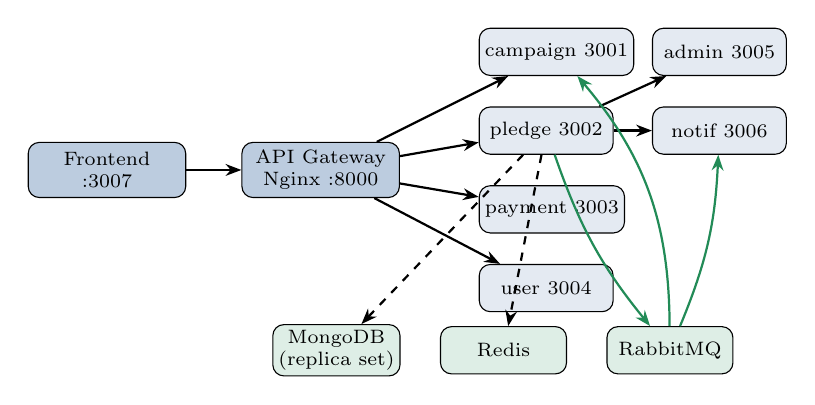
\begin{tikzpicture}[
      font=\scriptsize,
      box/.style={draw, rounded corners, fill=brandblue!12, minimum width=1.7cm, minimum height=0.6cm, align=center},
      infra/.style={draw, rounded corners, fill=brandgreen!15, minimum width=1.6cm, minimum height=0.6cm, align=center},
      gw/.style={draw, rounded corners, fill=brandblue!30, minimum width=2cm, minimum height=0.7cm, align=center},
      arr/.style={-{Stealth[length=2mm]}, thick}, every node/.style={inner sep=2pt}
    ]
    \node[gw] (fe) {Frontend\\:3007};
    \node[gw, right=0.7cm of fe] (gw) {API Gateway\\Nginx :8000};
    \node[box, right=1.0cm of gw, yshift=1.5cm] (c) {campaign 3001};
    \node[box, right=1.0cm of gw, yshift=0.5cm] (p) {pledge 3002};
    \node[box, right=1.0cm of gw, yshift=-0.5cm] (pay) {payment 3003};
    \node[box, right=1.0cm of gw, yshift=-1.5cm] (u) {user 3004};
    \node[box, right=3.2cm of gw, yshift=1.5cm] (a) {admin 3005};
    \node[box, right=3.2cm of gw, yshift=0.5cm] (n) {notif 3006};

    \node[infra, below=1.6cm of gw, xshift=0.2cm] (mongo) {MongoDB\\(replica set)};
    \node[infra, right=0.5cm of mongo] (redis) {Redis};
    \node[infra, right=0.5cm of redis] (mq) {RabbitMQ};

    \draw[arr] (fe) -- (gw);
    \foreach \t in {c,p,pay,u} {\draw[arr] (gw) -- (\t);}
    \draw[arr] (p) -- (a);
    \draw[arr] (p) -- (n);
    \draw[arr, brandgreen] (p) to[bend right=10] (mq);
    \draw[arr, brandgreen] (mq) to[bend right=20] (c);
    \draw[arr, brandgreen] (mq) to[bend right=10] (n);
    \draw[arr, dashed] (p) -- (mongo);
    \draw[arr, dashed] (p) -- (redis);
  \end{tikzpicture}
  \end{center}
  \vspace{-0.2em}
  \begin{itemize}\scriptsize
    \item Single base URL via gateway; clear service boundaries \& responsibilities.
    \item Green = asynchronous events (RabbitMQ); dashed = data/cache.
    \item Fault tolerance: a broker/consumer outage never loses a committed pledge.
  \end{itemize}
\end{frame}

% ---------------------------------------------------------------- CP1 data models + scaling
\begin{frame}{Checkpoint 1 --- Data models \& scalability}
  \begin{columns}[T]
    \begin{column}{0.52\textwidth}
      \textbf{Simple, clear models}
      \begin{itemize}\scriptsize
        \item \texttt{Campaign} + \texttt{CampaignTotals} (read model)
        \item \texttt{Pledge} (+ \texttt{donorReference}) + \texttt{Outbox}
        \item \texttt{Payment} (with \texttt{stateHistory}) + \texttt{WebhookEvent}
        \item \texttt{User}, \texttt{Notification}
      \end{itemize}
    \end{column}
    \begin{column}{0.48\textwidth}
      \textbf{Scalability (no orchestrator)}
      \begin{itemize}\scriptsize
        \item Horizontal scaling via Compose replicas
        \item Gateway re-resolves via Docker DNS $\Rightarrow$ round-robin LB
      \end{itemize}
      \begin{lstlisting}
docker compose \
 -f docker-compose.yml \
 -f docker-compose.scale.yml \
 up -d --scale pledge-service=5
      \end{lstlisting}
    \end{column}
  \end{columns}
  \vspace{0.3em}
  \begin{center}\scriptsize\good\ Demonstrated live: pledge=3, campaign=2, payment=2 replicas, gateway load-balanced.\end{center}
\end{frame}

% ---------------------------------------------------------------- Working flow
\begin{frame}{Working flow --- the donation pipeline}
  \begin{center}
  \begin{tikzpicture}[font=\scriptsize, node distance=0.55cm and 0.7cm,
      step/.style={draw, rounded corners, fill=brandblue!12, minimum width=2.2cm, minimum height=0.7cm, align=center},
      arr/.style={-{Stealth[length=2mm]}, thick}]
    \node[step] (s1) {1. POST /pledges\\(idempotencyKey)};
    \node[step, right=of s1] (s2) {2. Check Redis\\then Mongo};
    \node[step, right=of s2] (s3) {3. Tx: Pledge\\+ Outbox row};
    \node[step, below=of s3] (s4) {4. Worker polls\\Outbox (5s)};
    \node[step, left=of s4] (s5) {5. Publish\\pledge.created};
    \node[step, left=of s5] (s6) {6. Consumers:\\totals + notify};
    \draw[arr] (s1)--(s2); \draw[arr] (s2)--(s3); \draw[arr] (s3)--(s4);
    \draw[arr] (s4)--(s5); \draw[arr] (s5)--(s6);
  \end{tikzpicture}
  \end{center}
  \begin{itemize}\scriptsize
    \item Duplicate key (step 2) $\Rightarrow$ original pledge returned, \textbf{no double charge}.
    \item Pledge + event commit \textbf{atomically} (step 3) $\Rightarrow$ \textbf{no lost donations}.
    \item Read model \& notifications update from events (step 6) $\Rightarrow$ \textbf{fast, consistent totals}.
  \end{itemize}
\end{frame}

% ---------------------------------------------------------------- CP2 core
\begin{frame}{Checkpoint 2 --- Core implementation}
  \begin{itemize}
    \item All six services implemented with essential endpoints + inter-service events.
    \item Single base URL through the API gateway.
    \item \textbf{Unit tests (Jest) for every service} --- 8 suites, payment gateway covered thoroughly.
    \item Transparent donation history for \textbf{registered and unregistered} donors.
    \item Admin panel (role-gated) to manage \& monitor campaigns.
    \item \emph{Bonus:} notification service (event-driven).
    \item Dockerized; self-contained \texttt{docker-compose} the judges can run directly.
  \end{itemize}
  \vfill
  \begin{center}\scriptsize Next: the four reliability patterns that make it correct.\end{center}
\end{frame}

% ---------------------------------------------------------------- Pattern idempotency
\begin{frame}[fragile]{Pattern --- Idempotency (no double charge)}
  \begin{columns}[T]
    \begin{column}{0.55\textwidth}
      \begin{itemize}\small
        \item Client sends an \texttt{idempotencyKey}.
        \item Check \textbf{Redis} first, then \textbf{Mongo} fallback.
        \item Found $\Rightarrow$ return the \emph{original} result.
        \item Webhooks de-duplicated by \texttt{(provider, eventId)}.
      \end{itemize}
    \end{column}
    \begin{column}{0.45\textwidth}
      \begin{lstlisting}
const cached =
  await check(idempotencyKey);
if (cached) return existing;
// else create once, cache it
      \end{lstlisting}
    \end{column}
  \end{columns}
  \vspace{0.3em}
  \begin{center}\scriptsize\good\ Verified: two requests with the same key $\Rightarrow$ \emph{one} pledge.\end{center}
\end{frame}

% ---------------------------------------------------------------- Pattern outbox
\begin{frame}{Pattern --- Transactional Outbox (no lost events)}
  \begin{itemize}\small
    \item Pledge document \textbf{and} an \texttt{Outbox} row are written in \textbf{one MongoDB transaction}.
    \item A background worker polls every 5s, publishes \texttt{PENDING} events to RabbitMQ, marks them \texttt{PUBLISHED}.
    \item On failure: \texttt{retryCount++}; after 5 retries $\rightarrow$ \texttt{FAILED} (auditable).
  \end{itemize}
  \begin{center}\scriptsize
  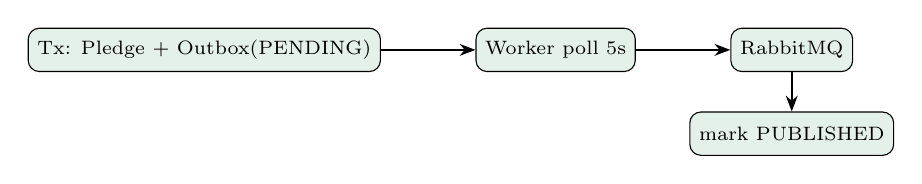
\begin{tikzpicture}[font=\scriptsize, node distance=0.5cm,
    b/.style={draw, rounded corners, minimum height=0.55cm, align=center, fill=brandgreen!12},
    arr/.style={-{Stealth[length=2mm]}, thick}]
    \node[b] (tx) {Tx: Pledge + Outbox(PENDING)};
    \node[b, right=1.2cm of tx] (w) {Worker poll 5s};
    \node[b, right=1.2cm of w] (mq) {RabbitMQ};
    \node[b, below=0.5cm of mq] (pub) {mark PUBLISHED};
    \draw[arr] (tx)--(w); \draw[arr] (w)--(mq); \draw[arr] (mq)--(pub);
  \end{tikzpicture}
  \end{center}
  \begin{center}\scriptsize\good\ Demonstrated: stop RabbitMQ $\rightarrow$ retries $\rightarrow$ restart $\rightarrow$ event published. No loss.\end{center}
\end{frame}

% ---------------------------------------------------------------- Pattern state machine
\begin{frame}{Pattern --- Payment State Machine (valid order only)}
  \begin{center}
  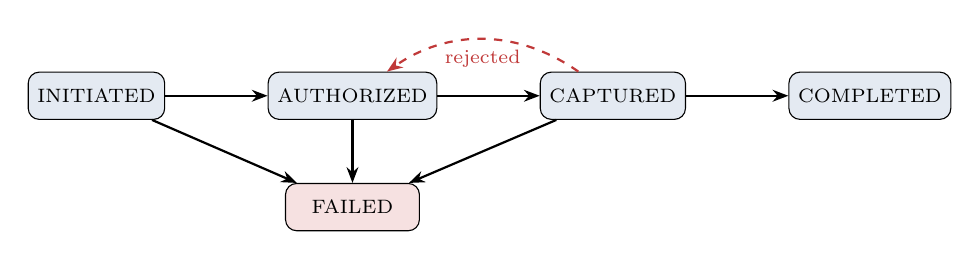
\begin{tikzpicture}[font=\scriptsize, node distance=1.3cm,
    s/.style={draw, rounded corners, fill=brandblue!12, minimum width=1.7cm, minimum height=0.6cm},
    t/.style={draw, rounded corners, fill=brandred!15, minimum width=1.7cm, minimum height=0.6cm},
    arr/.style={-{Stealth[length=2mm]}, thick}]
    \node[s] (i) {INITIATED};
    \node[s, right=of i] (a) {AUTHORIZED};
    \node[s, right=of a] (c) {CAPTURED};
    \node[s, right=of c] (co) {COMPLETED};
    \node[t, below=0.8cm of a] (f) {FAILED};
    \draw[arr] (i)--(a); \draw[arr] (a)--(c); \draw[arr] (c)--(co);
    \draw[arr] (i)--(f); \draw[arr] (a)--(f); \draw[arr] (c)--(f);
    \draw[-{Stealth[length=2mm]}, brandred, thick, dashed] (c) to[bend right=35] node[below]{rejected} (a);
  \end{tikzpicture}
  \end{center}
  \begin{itemize}\small
    \item Only forward transitions allowed; backward (CAPTURED $\rightarrow$ AUTHORIZED) is \textbf{rejected}.
    \item Terminal states: COMPLETED, FAILED. Every transition recorded in \texttt{stateHistory}.
    \item \good\ Unit-tested explicitly, including the original backward-transition bug.
  \end{itemize}
\end{frame}

% ---------------------------------------------------------------- Pattern CQRS + transparency
\begin{frame}{Pattern --- CQRS \& transparent histories}
  \begin{columns}[T]
    \begin{column}{0.5\textwidth}
      \textbf{CQRS read model}
      \begin{itemize}\scriptsize
        \item \texttt{CampaignTotals} materialized from events.
        \item Reads are O(1) lookups --- never recompute from scratch.
        \item Fixes the 100\% CPU / ``0 raised'' collapse.
      \end{itemize}
    \end{column}
    \begin{column}{0.5\textwidth}
      \textbf{Transparent histories}
      \begin{itemize}\scriptsize
        \item Registered: \texttt{GET /pledges/user/:id}
        \item Unregistered: \texttt{donorReference} +\\ \texttt{GET /pledges/reference/:ref}
        \item Anonymous pledges supported.
      \end{itemize}
    \end{column}
  \end{columns}
  \vspace{0.4em}
  \begin{center}\scriptsize\good\ Verified: totals update via events; guest retrieves full history by reference.\end{center}
\end{frame}

% ---------------------------------------------------------------- CP3 Observability
\begin{frame}{Checkpoint 3 --- Observability \& monitoring}
  \begin{columns}[T]
    \begin{column}{0.33\textwidth}
      \textbf{Metrics}
      \begin{itemize}\scriptsize
        \item Prometheus + Grafana
        \item cAdvisor (containers)
        \item Node Exporter (host)
        \item All 9 targets \texttt{up}
      \end{itemize}
    \end{column}
    \begin{column}{0.33\textwidth}
      \textbf{Logging}
      \begin{itemize}\scriptsize
        \item Logstash $\rightarrow$ Elasticsearch
        \item Kibana dashboards
        \item Structured per-service logs
      \end{itemize}
    \end{column}
    \begin{column}{0.33\textwidth}
      \textbf{Tracing}
      \begin{itemize}\scriptsize
        \item OpenTelemetry
        \item Jaeger end-to-end traces
        \item Full donation workflow
      \end{itemize}
    \end{column}
  \end{columns}
  \vspace{0.4em}
  \textbf{Demonstrated scenarios}
  \begin{itemize}\scriptsize
    \item End-to-end trace of a donation in Jaeger.
    \item \textbf{Stress test} (\texttt{scripts/stress-test.ps1}) --- watch CPU/latency under load.
    \item \textbf{Partial failure}: RabbitMQ down $\rightarrow$ outbox retries $\rightarrow$ recovery on restart.
  \end{itemize}
\end{frame}

% ---------------------------------------------------------------- CP4 CI/CD
\begin{frame}{Checkpoint 4 --- CI/CD pipeline}
  \begin{center}
  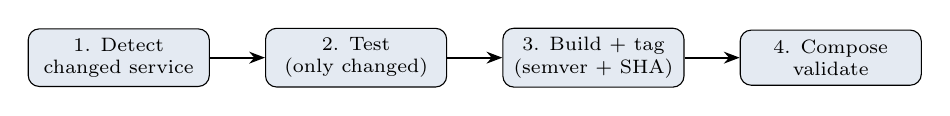
\begin{tikzpicture}[font=\scriptsize, node distance=0.7cm,
    b/.style={draw, rounded corners, fill=brandblue!12, minimum width=2.3cm, minimum height=0.7cm, align=center},
    arr/.style={-{Stealth[length=2mm]}, thick}]
    \node[b] (ch) {1. Detect\\changed service};
    \node[b, right=of ch] (te) {2. Test\\(only changed)};
    \node[b, right=of te] (bu) {3. Build + tag\\(semver + SHA)};
    \node[b, right=of bu] (cd) {4. Compose\\validate};
    \draw[arr] (ch)--(te); \draw[arr] (te)--(bu); \draw[arr] (bu)--(cd);
  \end{tikzpicture}
  \end{center}
  \begin{itemize}\small
    \item GitHub Actions; runs on every PR / push to \texttt{main}.
    \item \textbf{Change detection} (\texttt{dorny/paths-filter}) --- test/build \emph{only} the changed service.
    \item \textbf{Semantic versioning} per service; images tagged with version + commit SHA.
    \item Branch protection gates merges on passing CI.
  \end{itemize}
\end{frame}

% ---------------------------------------------------------------- Scaling
\begin{frame}{Scaling --- bursts beyond 1000 req/s}
  \begin{itemize}\small
    \item No \texttt{container\_name} on app services $\Rightarrow$ Compose can run N replicas.
    \item Gateway resolves service names at request time (Docker DNS) $\Rightarrow$ automatic round-robin.
    \item \texttt{docker-compose.scale.yml} sets replica counts and frees host ports.
  \end{itemize}
  \begin{center}\scriptsize
  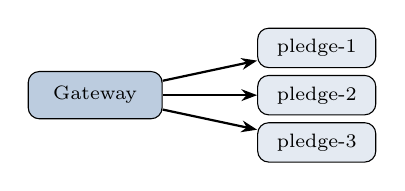
\begin{tikzpicture}[font=\scriptsize, node distance=0.45cm,
    b/.style={draw, rounded corners, fill=brandblue!12, minimum width=1.5cm, minimum height=0.5cm},
    g/.style={draw, rounded corners, fill=brandblue!30, minimum width=1.7cm, minimum height=0.6cm},
    arr/.style={-{Stealth[length=2mm]}, thick}]
    \node[g] (gw) {Gateway};
    \node[b, right=1.2cm of gw, yshift=0.6cm] (r1) {pledge-1};
    \node[b, right=1.2cm of gw] (r2) {pledge-2};
    \node[b, right=1.2cm of gw, yshift=-0.6cm] (r3) {pledge-3};
    \draw[arr] (gw)--(r1); \draw[arr] (gw)--(r2); \draw[arr] (gw)--(r3);
  \end{tikzpicture}
  \end{center}
  \begin{center}\scriptsize\good\ Proven live; traffic served across replicas with no config change.\end{center}
\end{frame}

% ---------------------------------------------------------------- Verification
\begin{frame}{Verification \& results}
  \begin{table}\centering\small
    \begin{tabular}{@{}ll@{}}
      \toprule
      Check & Result \\
      \midrule
      Unit tests (Jest, 6 services) & \good\ 8 suites passing \\
      Idempotency (same key) & \good\ one pledge, no duplicate \\
      Transactional outbox & \good\ event survives broker outage \\
      State machine & \good\ backward transition rejected \\
      CQRS totals & \good\ updated via events \\
      Notifications & \good\ created from events \\
      Scaling (replicas) & \good\ gateway load-balanced \\
      Observability targets & \good\ 9/9 Prometheus targets up \\
      \bottomrule
    \end{tabular}
  \end{table}
  \begin{center}\scriptsize One-command checks: \texttt{scripts/feature-test.ps1}, \texttt{scripts/stress-test.ps1}.\end{center}
\end{frame}

% ---------------------------------------------------------------- Continuity recap
\begin{frame}{Continuity --- how the checkpoints connect}
  \begin{center}
  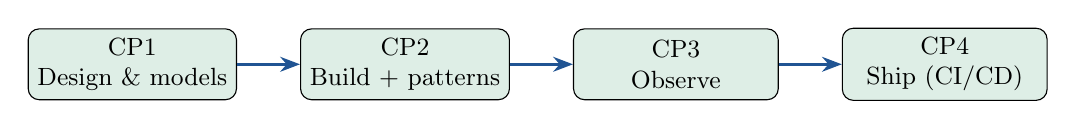
\begin{tikzpicture}[font=\small, node distance=0.8cm,
    b/.style={draw, rounded corners, fill=brandgreen!15, minimum width=2.6cm, minimum height=0.9cm, align=center},
    arr/.style={-{Stealth[length=2.5mm]}, very thick, brandblue}]
    \node[b] (d) {CP1\\Design \& models};
    \node[b, right=of d] (i) {CP2\\Build + patterns};
    \node[b, right=of i] (o) {CP3\\Observe};
    \node[b, right=of o] (c) {CP4\\Ship (CI/CD)};
    \draw[arr] (d)--(i); \draw[arr] (i)--(o); \draw[arr] (o)--(c);
  \end{tikzpicture}
  \end{center}
  \begin{itemize}\small
    \item \textbf{Design} defined the boundaries that made each pattern possible.
    \item \textbf{Implementation} turned every past failure into a tested guarantee.
    \item \textbf{Observability} makes that correctness \emph{visible} and debuggable.
    \item \textbf{CI/CD} keeps it correct as the system evolves --- per-service, versioned.
  \end{itemize}
\end{frame}

% ---------------------------------------------------------------- Conclusion
\begin{frame}{Conclusion}
  \begin{itemize}
    \item The old platform failed on foundations --- we rebuilt those foundations.
    \item Idempotency, outbox, state machine, CQRS, retries, observability --- all implemented \emph{and} verified.
    \item Self-contained, scalable, observable, and shipped through a real CI/CD pipeline.
  \end{itemize}
  \vfill
  \begin{center}
    \Large\textcolor{brandblue}{Thank you --- questions?}\\[0.4em]
    \small Run it: \texttt{docker compose up -d} $\rightarrow$ \texttt{http://localhost:3007}
  \end{center}
\end{frame}

\end{document}
